\documentclass{article}
\usepackage{iclr2025_conference}
\usepackage{times}
\usepackage{natbib}
\usepackage{booktabs}
\usepackage{amsmath,amssymb}
\usepackage{graphicx}
\usepackage{xcolor}
\usepackage{hyperref}
\usepackage{multirow}

% --- TODO marker -------------------------------------------------------------
\newcommand{\todo}[1]{\textcolor{red}{[TODO: #1]}}

% --- Method name macros ------------------------------------------------------
\newcommand{\method}{T-DSO}        % transcoder-guided variant
\newcommand{\methodfree}{T-DSO$_{\text{free}}$} % dictionary-free variant (native MLP basis)
\newcommand{\baseline}{TaCQ}

\title{Conjunctive Task-Circuit Saliency for Low-Bit LLM Quantization}

\author{Anonymous Authors\\
\texttt{anonymous@domain.edu}}

\begin{document}
\maketitle

\begin{abstract}
Low-bit post-training quantization (PTQ) compresses large language models but
often destroys task-specific capabilities when only a tiny fraction of weights
can remain in full precision. Task-Circuit Quantization (\baseline{}) selects
FP16 outlier weights using contrastive gradients on cross-entropy loss,
treating the model as a black box. We propose \emph{conjunctive task-circuit
saliency}: a weight is protected only if it is salient \emph{both} to the task
loss \emph{and} to the activation circuit that distinguishes clean from
corrupted task inputs. We instantiate the circuit term in two bases: sparse
transcoder features (\method{}) and---crucially---the model's \emph{own MLP
neurons} (\methodfree{}), which requires no external dictionary and applies to
any transformer. A controlled saliency-source ablation on Llama-3.1-8B-Instruct
(matched 0.35\% FP16 budget, identical GPTQ pipeline, only the saliency signal
varies) shows at 2-bit: (i) circuit-informed selection far exceeds magnitude,
quantization-error, and random controls; (ii) the conjunction beats either of
its parts (GSM8K: 28.7\% vs.\ CE 25.4\% and circuit-only 25.6\%); and (iii) the
dictionary is \emph{optional}: \methodfree{} recovers most of the transcoder
gain on GSM8K (26.5\%) and surpasses all transcoder arms on MMLU-STEM (44.2\%
vs.\ 38.9\%). At 3-bit all task-conditioned methods converge, identifying
conjunctive saliency as a distinctly \emph{low-bit} phenomenon: where to spend
the FP16 budget matters most exactly when the budget is harshest. On Spider
text-to-SQL, \method{} v2~mult improves execution accuracy by +2.9 points on
average over four paired calibration seeds (29.4\% vs.\ \baseline{} 26.5\%).
\end{abstract}

\section{Introduction}
\label{sec:intro}

Large language models (LLMs) are increasingly deployed under strict memory and
latency budgets. Post-training quantization (PTQ) maps FP16 weights to 2--4
bits without retraining, but aggressive quantization---especially at 2
bits---can collapse performance on structured tasks such as text-to-SQL, math
reasoning, and code generation. Mixed-precision PTQ mitigates this by keeping a
small set of outlier weights in FP16 while quantizing the
rest~\citep{dettmers2022llmint8,frantar2023gptq,dettmers2023spqr}.

\paragraph{The core problem.}
Outlier selection is a \emph{localization} problem: which weights matter for a
downstream task once quantization noise is injected? Uniform salience
heuristics (magnitude, activation scale) ignore task structure. Calibration on
generic corpora misses task-specific circuits. Even strong mixed-precision
methods struggle in the 2-bit regime, where the allowed FP16 budget (often
$<$1\% of weights) must be spent with surgical precision.

\paragraph{Polysemantic weights vs.\ monosemantic features.}
A separate challenge is \emph{where} in the network task signal lives.
Individual MLP neurons and their connecting weights are typically
polysemantic---each participates in many unrelated computations via
superposition~\citep{elhage2021mathematical,bricken2023monosemanticity}. A
gradient on cross-entropy therefore reflects a mixture of all roles a weight
plays across the vocabulary and prompt positions, not a single task-specific
mechanism. \baseline{} inherits this ambiguity: although it conditions on task
calibration data, saliency is still computed directly on physical weights from
CE gradients, so the selected outliers may protect broadly useful directions
rather than the sparse features that implement SQL grounding, aggregation, or
schema linking.

\paragraph{Task-Circuit Quantization (\baseline{}).}
\citet{xiao2025tacq} frame outlier selection as automated circuit discovery for
PTQ. They score each weight by combining (i) contrastive gradients on task
calibration data, (ii) expected weight change under quantization
$\Delta W = W - W_{\text{quant}}$, and (iii) a global top-$p$ mask under a
fixed memory budget. Crucially, \baseline{} operates in weight space on
polysemantic gradient signal; it does not decompose MLP computation into
features before ranking outliers.

\paragraph{Step 1 --- \method{}: route saliency through a monosemantic basis.}
Our starting point is interpretability-guided: if CE gradients on weights are
polysemantic, attribute through a basis that is not. \method{}
(Transcoder-guided Dynamic Sparse Overlay) uses sparse TopK
transcoders~\citep{dunefsky2024transcoders} to identify features that activate
preferentially on task-faithful versus corrupted inputs, back-propagates a
feature-filtered reconstruction objective, and \emph{intersects} the resulting
circuit saliency with standard CE saliency (geometric mean;
\S\ref{sec:method}). This works: +2.9 points mean Spider execution accuracy
over four paired seeds and +3.3 points GSM8K at 2-bit versus \baseline{} at
matched budget, with the selected mask sharing only $J{=}0.30$ of its weights
with \baseline{}'s.

\paragraph{Step 2 --- dissect it: which ingredient carries the gain?}
A method with three coupled ingredients (contrastive circuit localization, a
pretrained transcoder dictionary, and a conjunction rule) invites the question
of what is actually doing the work---and transcoders exist only for a handful
of models, which would cap the method's reach. We therefore run a
\emph{saliency-source ablation} in which everything is held fixed (model,
0.35\% budget, contrastive pairs, GPTQ, evaluation) and only the signal that
ranks weights varies across eight arms: random, weight magnitude $|W|$,
magnitude $\times$ quantization error $|W|\cdot|\Delta W|$, CE
($\approx$\baseline{}), circuit-only, and the conjunction---each circuit arm
instantiated in \emph{two} bases: the transcoder and, replacing it, the
model's \emph{own MLP neurons} with \texttt{down\_proj} as the decoder.

\paragraph{Step 3 --- the distilled method: \methodfree{}.}
The ablation delivers a clean dissection: the conjunction is the active
ingredient, and the dictionary is not. The native-basis conjunction
(\methodfree{}) recovers most of \method{}'s gain on GSM8K and surpasses it on
MMLU-STEM, while requiring no external dictionary, SAE, or transcoder---the
method applies out-of-the-box to any transformer. What began as a
transcoder-dependent technique ends as a general principle: \emph{protect a
weight only if it is salient to both the task loss and the task circuit; any
sufficiently task-discriminative feature basis---including the model's
own---suffices to define the circuit.}

\paragraph{Contributions.}
\begin{itemize}
  \item \textbf{\method{}:} we introduce transcoder-guided outlier selection
        for PTQ---routing saliency through task-discriminative monosemantic
        features and intersecting with CE---and show it beats \baseline{} at
        matched budget on Spider (+2.9\,pp mean over four paired seeds) and
        GSM8K 2-bit (+3.3\,pp), with interpretability analysis showing low
        mask overlap ($J{=}0.30$) and causal knockout ($-29$\,pt).
  \item \textbf{Dissection:} a controlled eight-arm saliency-source ablation
        isolates the active ingredient. Task-circuit information dominates
        magnitude/error/random placement by 10--26 points at 2-bit, and the
        \emph{conjunction} beats both of its parts (GSM8K: 28.7\% vs.\ CE
        25.4\% / circuit-only 25.6\%; \S\ref{sec:ablation}).
  \item \textbf{\methodfree{}:} the dissection shows the dictionary is
        optional. Using the model's own MLP neurons as the circuit basis
        recovers most of the transcoder gain on GSM8K and \emph{surpasses} it
        on MMLU-STEM (44.2\% vs.\ 38.9\%), removing the dependency on external
        interpretability artifacts and extending task-circuit PTQ to any
        transformer.
  \item \textbf{Regime analysis:} all task-conditioned methods converge at
        3-bit; conjunctive saliency is a \emph{low-bit} phenomenon
        (\S\ref{sec:results-3bit}), locating exactly where saliency choice
        matters.
  \item We release code, contrastive calibration sets, and reproduction
        scripts for \baseline{}, \method{}, and \methodfree{} masks.
        \todo{anonymize for submission}
\end{itemize}

\paragraph{Paper roadmap.}
Section~\ref{sec:encoded-used} gives the theoretical framing;
Section~\ref{sec:rqs} states research questions;
Section~\ref{sec:related} situates our work;
Section~\ref{sec:method} describes the algorithm and the dictionary-free
variant; Sections~\ref{sec:setup}--\ref{sec:results} cover setup and findings.

\section{Theoretical Framing: Encoded--Used Gap Dissociation}
\label{sec:encoded-used}

We frame \method{} against \baseline{} as a \emph{targeted scalpel} vs.\ a \emph{global broadsword}.
Both preserve a tiny FP16 outlier budget under mixed-precision GPTQ; they differ in \emph{what signal
selects} those outliers.

\paragraph{The encoded--used ambiguity in \baseline{}.}
Cross-entropy on final logits conflates two roles of weights in text-to-SQL:
\begin{itemize}
  \item \textbf{Encoding:} weights that store schema syntax, SQL templates, and lexical priors
        (often active whenever SQL-like tokens appear).
  \item \textbf{Using:} weights on causal execution edges---routing that binds columns, applies
        aggregations, and composes structure for the \emph{current} question.
\end{itemize}
Because CE gradients flow through the full vocabulary, \baseline{}'s contrastive saliency still
 mixes encoding and use under a single polysemantic ranking~\citep{xiao2025tacq}.
At 0.35\% outliers, wasting budget on passive encoders directly costs execution accuracy on Spider.

\paragraph{Dissociation via $F_{\text{task}}$.}
\method{} selects transcoder features with $\Delta a = \mathrm{ReLU}(a_{\text{clean}} - a_{\text{corr}}) > \tau$
and builds $y^{\text{target}}$ only from this task set $F_{\text{task}}$.
Gradients therefore align with weights that implement \emph{contrastive, task-active} MLP directions,
not every pathway that lowers CE on SQL surface form.
We call this \textbf{encoded--used gap dissociation}: outliers target active routing momentum rather
than undifferentiated static memory.
\todo{Cite feature-level audit or layer analysis supporting dissociation.}

\paragraph{What we claim in v1 vs.\ systems extensions.}
\textbf{v1 (this paper):} same static mask, same quantizer, same budget as \baseline{}; test whether
dissociation improves Spider execution accuracy at 2--3 bits.
\textbf{Extensions (outlook, \S\ref{sec:systems-outlook}):} distinct sub-task masks, orthogonality
constraints, and KV-cache-preserving hot-swaps---architectural capabilities \baseline{}'s static
monolith cannot express.

\section{Research Questions}
\label{sec:rqs}

\paragraph{RQ1: Conjunctive vs.\ single-signal saliency.}
Does requiring a weight to be salient to both the task loss \emph{and} the
task circuit identify a better outlier set than either signal alone at the
same FP16 budget?
\emph{Status:} Yes at 2-bit. Ablation (Table~\ref{tab:ablation}): mult 28.7\%
vs.\ ce 25.4\% / align 25.6\% on GSM8K; mult$_{\text{free}}$ 44.2\% vs.\ ce
41.3\% / align$_{\text{free}}$ 42.6\% on MMLU-STEM. Spider: v2~mult
$+2.9$\,pp mean over four paired seeds (Table~\ref{tab:spider}).

\paragraph{RQ2: Is an external dictionary necessary?}
Can the circuit term be computed in the model's native MLP-neuron basis
without transcoders or SAEs?
\emph{Status:} Yes. \methodfree{} recovers 92\% of the transcoder gain on
GSM8K and surpasses all transcoder arms on MMLU-STEM
(\S\ref{sec:ablation}). The dictionary is an optional booster, not a
dependency.

\paragraph{RQ3: Circuit vs.\ bit-placement heuristics.}
Do magnitude, quantization-error, and random selection explain the gains?
\emph{Status:} No. Controls trail circuit-informed arms by 10--26 points at
2-bit on GSM8K and sit near chance on MMLU-STEM (Table~\ref{tab:ablation}).

\paragraph{RQ4: Bit-width dependence.}
At what quantization severity does saliency choice matter?
\emph{Status:} Conjunctive saliency is a low-bit phenomenon: decisive at
2-bit, within seed noise at 3-bit (\S\ref{sec:results-3bit}).

\paragraph{RQ5: Feature--weight alignment under superposition.}
Do task-discriminative circuit features map to distinct weight subsets from CE
saliency?
\emph{Status:} $J{=}0.298$ (2-bit) / 0.331 (3-bit) between v2~mult and
\baseline{}; mid layers 4--14 and MLP projections diverge most; cross-seed
stability $J{=}0.995$--0.997 (v2) vs.\ 0.983--0.985 (\baseline{})
(\S\ref{sec:analysis-overlap}).

\paragraph{RQ6: Calibration source.}
How much does the calibration distribution matter at 2--3 bit?
\emph{Status:} A 25+ point collapse when switching \baseline{} MSG from Spider
to C4 calibration at 2-bit (\S\ref{sec:domain-shift}); task-matched
calibration is necessary even with the mask held fixed.

\paragraph{RQ7: Baseline reproduction.}
Does our ported \baseline{} pipeline behave consistently with published
numbers? \emph{Status:} Llama-3-8B Spider replication matches paper targets
(67.7 / 22.3 / 60.1 exec\%).

\section{Related Work}
\label{sec:related}

\paragraph{Post-training quantization.}
GPTQ~\citep{frantar2023gptq} remains the workhorse for weight-only PTQ of LLMs.
Activation-aware methods (AWQ~\citep{lin2024awq}), omnidirectional calibration
(OmniQuant~\citep{shao2024omniquant}), and 2-bit specialized schemes
(QuIP\#~\citep{chee2024quip}) improve uniform quantization but still degrade on hard reasoning
tasks at 2 bits.
Mixed-precision and sparse formats---LLM.int8()~\citep{dettmers2022llmint8},
SPQR~\citep{dettmers2023spqr}, SliM-LLM~\citep{huang2025slimllm}---retain high-magnitude or
salient weights in higher precision via magnitude, Hessian, or group-wise bit allocation.
ReALLM~\citep{bedin2025reallm} compresses each weight matrix with a residual autoencoder plus
vector quantization---a different architectural decomposition, not task-conditioned outlier
selection.
These methods generally define salience without an explicit \emph{task-circuit} or
\emph{monosemantic feature} basis.

\paragraph{Task-conditioned mixed precision.}
\baseline{}~\citep{xiao2025tacq} is the closest prior work to ours.
Presented at COLM 2025, it uses contrastive calibration, quantization-aware localization (QAL)
and magnitude-sharpened gradients (MSG) with a global top-$p$ mask, explicitly connecting PTQ to
automated circuit discovery and knowledge localization~\citep{conmy2023automated}.
Across QA, math, and text-to-SQL on Llama-3 and Qwen2.5, \baseline{} outperforms SPQR and
SliM-LLM at matched bit budgets---especially at 2--3 bits.
We treat \baseline{} as the primary baseline because it shares our GPTQ stack, $\Delta W$ corrupt
model, outlier fraction (0.35\%), and Spider evaluation protocol.
However, \baseline{} scores \emph{polysemantic weights} via CE on logits; \method{} intersects CE
with saliency routed through a monosemantic transcoder basis (\S\ref{sec:method}).
Empirically, our v2 \texttt{mult} mask overlaps only 30\% (Jaccard $J{=}0.298$) with \baseline{} at the same
budget (\S\ref{sec:mask-overlap}), showing the gain is not a minor reranking within \baseline{}'s
weight pool.

\paragraph{Superposition, polysemanticity, and sparse features.}
\citet{elhage2021mathematical} argue that capacity constraints force LLMs to encode more features
than neurons, yielding \emph{polysemantic} units whose activations mix many concepts.
Dictionary learning and sparse autoencoders (SAEs) recover latents closer to
\emph{monosemanticity}---each feature aligns with a narrower behavior~\citep{bricken2023monosemanticity,cunningham2024sparse}.
Transcoders apply the same idea at MLP boundaries: they approximate $\mathrm{MLP}(x)$ with a
wider, sparsely activating layer~\citep{dunefsky2024transcoders}, enabling cleaner circuit
factorization than residual-stream SAEs~\citep{wright2025transcodersbeat}.
Prior work uses these tools for \emph{analysis}, steering, or verification
(\S\ref{sec:related-steering}); we ask whether monosemantic feature attribution should
\emph{drive compression} by deciding which polysemantic weights must remain in FP16.

\paragraph{Mechanistic interpretability, transcoders, and circuit verification.}
Transformer circuits~\citep{elhage2021mathematical} and automated circuit discovery~\citep{conmy2023automated}
seek sparse subgraphs explaining behaviors.
Meta's Circuit Tracer and the public \texttt{crv-8b-instruct-transcoders} weights provide
per-layer TopK transcoders for Llama-3.1-8B-Instruct~\citep{crv2026}.
Circuit-based Reasoning Verification (CRV)~\citep{crv2026} replaces MLPs with these transcoders
to build attribution graphs, classify reasoning errors, and intervene on individual features---the
same sparse basis we use, but for \emph{runtime verification} rather than \emph{offline weight
selection}.
Unlike \baseline{}, which ranks polysemantic weights from CE gradients, \method{} attributes through
this monosemantic feature basis first, then maps saliency back to physical parameters.

\paragraph{Sparse-feature steering and contrastive attribution.}
\label{sec:related-steering}
Contrastive prompts (clean vs.\ corrupted inputs) appear in influence estimation, data attribution,
and \baseline{}'s gradient capture.
Sparse Activation Steering (SAS)~\citep{bayat2025sas}, also at COLM 2025, uses contrastive
prompt pairs to isolate behavior-specific SAE latents and steer model activations at inference---
sharing our motivation to escape superposition, but modifying \emph{activations} at test time
rather than selecting \emph{weights} at compression time.
SAE-Targeted Steering~\citep{chalnev2024saets} constructs steering vectors by modeling effects on
SAE features; again, the output is a steering direction, not a quantization mask.
We reuse contrastive calibration infrastructure but change \emph{what is being attributed}:
transcoder feature activations on MLP hooks (and their intersection with CE), combined with
$|W|\cdot|\Delta W|$ as in \baseline{}.

\paragraph{Quantization vs.\ interpretability.}
Recent work studies how PTQ \emph{damages} SAE features even when perplexity looks stable~\citep{quantfeatures2026},
motivating feature-level audits of compressed models.
Our direction is complementary: we use interpretability tools \emph{upstream} to choose a mask that
preserves task performance, then measure whether the selected circuit differs from CE-only selection.

\paragraph{Text-to-SQL as a testbed.}
Spider~\citep{yu2018spider} is a standard semantic parsing benchmark requiring schema grounding
and compositional SQL.
It stress-tests structured output under quantization and matches \baseline{}'s headline results.
We extend evaluation to \todo{GSM8K, HumanEval} for generality.

\paragraph{Positioning.}
Table~\ref{tab:positioning} summarizes how \method{} relates to the closest lines of work.
To our knowledge, no prior conference paper uses transcoder (or SAE) task-feature attribution to
select PTQ outlier \emph{weights} under a fixed FP16 budget and reports both (i)~downstream task
gains vs.\ \baseline{} and (ii)~low mask overlap showing a distinct circuit.
\method{} sits at the intersection of \emph{task-aware PTQ}~\citep{xiao2025tacq,huang2025slimllm}
and \emph{monosemantic feature attribution}~\citep{dunefsky2024transcoders,bayat2025sas,crv2026}.
Unlike \baseline{}, we do not treat weights as atomic units of task importance---we decompose MLP
computation to mitigate polysemanticity before selecting outliers.
Unlike steering and verification work, we do not seek human-readable explanations or runtime control
for their own sake---we convert feature-level task signal into a weight mask with measurable
downstream impact (+3.4\,pt mean Spider exec at 2-bit vs.\ \baseline{}, four seeds;
\S\ref{sec:seed-robustness}).

\begin{table}[t]
  \centering
  \caption{Positioning vs.\ closest prior work (all target low-bit LLM compression or control).}
  \label{tab:positioning}
  \small
  \begin{tabular}{@{}p{0.22\linewidth}p{0.18\linewidth}p{0.28\linewidth}c@{}}
    \toprule
    Method & Goal & Feature basis & Weights? \\
    \midrule
    SPQR / AWQ / SliM-LLM & PTQ & Magnitude / Hessian / salience & \checkmark \\
    \baseline{}~\citep{xiao2025tacq} & Task PTQ & CE (polysemantic) & \checkmark \\
    SAS / SAE-TS~\citep{bayat2025sas,chalnev2024saets} & Steer & SAE latents & --- \\
    CRV~\citep{crv2026} & Verify CoT & Transcoder latents & --- \\
    \method{} (ours) & Task PTQ & Transcoder $\cap$ CE & \checkmark \\
    \bottomrule
  \end{tabular}
\end{table}

\section{Method: Conjunctive Task-Circuit Saliency}
\label{sec:method}

We keep the \baseline{} mixed-precision quantization pipeline (GPTQ with
per-weight bit-width mask) and replace only the saliency extraction stage.

\paragraph{Setup.}
Model $f_\theta$ with weights $\theta$; uniform $b$-bit reference
$W_{b\text{bit}}$ (RTN or GPTQ on task calibration data); outlier budget $k$
(fraction of parameters kept in FP16, 0.35\% throughout). Contrastive pairs
$(x^+, x^-)$ where $x^+$ is task-faithful and $x^-$ is corrupted (schema
errors, wrong CoT, wrong answer choice, etc.).

\paragraph{\baseline{} saliency (review).}
Accumulate $|\nabla_W \mathcal{L}_{\text{CE}}(x^+)|$ over calibration, multiply
by $|W| \cdot |W - W_{b\text{bit}}|$, global top-$k$
selection~\citep{xiao2025tacq}. Gradients are taken w.r.t.\ polysemantic
weight tensors: each $W$ may contribute to many superposed features, and
$\mathcal{L}_{\text{CE}}$ mixes all roles active at each token.

\subsection{Circuit saliency in a feature basis}
\label{sec:method-circuit}

The circuit term inserts a feature-space bottleneck before weight saliency.
For each layer $\ell$, an encoder maps the MLP computation to a code
$f \in \mathbb{R}^{F_\ell}$; a decoder $D_\ell$ maps codes back to the MLP
output space. We rank \emph{task-discriminative} features via contrastive
activation: on corrupted input $x^-$ (no grad) record
$a^{\text{corr}}_{\ell,f} = \max_t f_{\ell,t,f}$; on clean input $x^+$ (with
grad) compute $a^{\text{clean}}_{\ell,f}$ analogously. Task features satisfy
\begin{equation}
\Delta a_\ell \;=\; \mathrm{ReLU}\!\left(a^{\text{clean}}_\ell - a^{\text{corr}}_\ell\right) \;>\; \tau_\ell,
\end{equation}
with $\tau_\ell$ the per-example 95th percentile of positive $\Delta a$. The
target MLP output contribution is
$y^{\text{target}}_\ell = D_\ell\!\left(f^{\text{clean}}_\ell \odot \mathbf{1}_{\Delta a > \tau}\right)$,
and the per-layer alignment loss is
$\mathcal{L}_\ell = -\sum_t \langle h^{\text{mlp,out}}_{\ell,t},\, y^{\text{target}}_{\ell,t} \rangle$.
One backward pass over $\mathcal{L} = \sum_\ell \mathcal{L}_\ell$ accumulates
$|\nabla_W \mathcal{L}|$ (\texttt{sample\_abs} semantics, matching
\baseline{}). Only weights on paths that implement the selected
task-discriminative features receive gradient; polysemantic CE would
additionally reward weights tied to non-task features active at the same
tokens.

\paragraph{Basis 1: transcoders (\method{}).}
$F_\ell \gg d_{\text{mlp}}$ sparse TopK transcoder features
(\texttt{facebook/crv-8b-instruct-transcoders}; $F{=}131{,}072$), whose entries
are approximately
monosemantic~\citep{bricken2023monosemanticity,dunefsky2024transcoders}. This
basis offers the cleanest feature separation but exists only for models with a
published dictionary.

\paragraph{Basis 2: native MLP neurons (\methodfree{}, dictionary-free).}
\label{sec:method-dictfree}
We take the model's own MLP hidden layer as the feature basis: the
post-activation intermediate
$f_{\ell} = \sigma(W_{\text{gate}} x) \odot (W_{\text{up}} x) \in \mathbb{R}^{d_{\text{mlp}}}$
serves as the code, and the model's own \texttt{down\_proj} matrix is the
decoder $D_\ell$. The contrastive selection rule and alignment loss are
\emph{identical} to the transcoder case; only the basis changes.

\emph{Intuition.} Individual MLP neurons are more polysemantic than dictionary
features, so each selected neuron is a noisier task indicator. But the
contrastive $\Delta a$ filter operates at the \emph{population} level: neurons
that consistently fire more on clean than corrupted task inputs are, in
aggregate, enriched for the task circuit even if no single neuron is
monosemantic. Because the conjunction with CE saliency (below) demotes weights
that only one signal favors, residual polysemantic noise in the circuit term
is filtered rather than propagated into the mask. Empirically this native
basis recovers most of the transcoder's gain on GSM8K and surpasses it on
MMLU-STEM (\S\ref{sec:ablation})---the dictionary is an optional booster, not a
requirement. \methodfree{} thus applies to \emph{any} transformer with no
external artifacts, removing the main practical barrier to task-circuit PTQ.

\subsection{Conjunctive combination and mask}
\label{sec:method-conjunction}

For each weight tensor $W$, define per-weight CE saliency $g_{\text{CE}}$ as in
\baseline{} and circuit saliency $g_{\text{align}}$ from $\mathcal{L}$ above
(same $|W|$ and $|W - W_{b\text{bit}}|$ scaling). Our main variant
(\texttt{mult}) combines both via geometric mean:
\begin{equation}
\label{eq:mult}
S(W) \;=\; |W| \cdot |W - W_{b\text{bit}}| \cdot \sqrt{g_{\text{CE}}(W)\, g_{\text{align}}(W)},
\end{equation}
selecting weights salient under \emph{both} task loss and task circuit. The
conjunction is the active ingredient: replacing $g_{\text{CE}}$ entirely with
$g_{\text{align}}$ (\texttt{align}) or using CE alone ties or trails on every
task we test, and union-style boosts
($g_{\text{CE}}(1 + \lambda g_{\text{align}})$) degenerate at 2-bit
(\S\ref{sec:ablation}). Global top-$k$ over all eligible linear weights yields
the binary mask $M$; GPTQ quantizes $M(W){=}0$ to $b$-bit and keeps
$M(W){=}1$ in FP16.

\paragraph{Why the conjunction works at low bit-width.}
At 2-bit, quantization noise is large enough that protecting the wrong weights
has a first-order cost: budget spent on weights that merely \emph{encode}
generic surface statistics (high CE saliency, low circuit saliency) or on
circuit edges whose quantization error happens to be benign (high circuit, low
CE) is budget taken from weights that are both functionally necessary and
fragile. The geometric mean implements an AND-gate over the two failure modes.
At 3-bit the noise floor drops and nearly any sensible task-conditioned mask
suffices---which is exactly what we observe (\S\ref{sec:results-3bit}).

\subsection{Anchored union: consensus core and dispute region}
\label{sec:method-anchored}

Empirically, \baseline{} and v2~mult agree on only ${\sim}46$--$50\%$ of the
FP16 budget ($J{\approx}0.30$--$0.33$; \S\ref{sec:analysis-overlap}). We
formalize a two-region policy that never renegotiates consensus outliers and
allocates only the remaining budget on the method-disputed mass. Let $\Omega$
be the eligible weight indices, $s_{\text{\baseline{}}}(w)$ and
$s_{\text{\method{}}}(w)$ the final per-weight scores, and
$k = \lfloor \rho |\Omega| \rfloor$, $\rho{=}0.0035$. Each method induces a
mask by global top-$k$; define
$M_{\text{core}} \triangleq M_{\text{\baseline{}}} \cap M_{\text{\method{}}}$
and
$M_{\text{dispute}} \triangleq M_{\text{\baseline{}}} \,\triangle\, M_{\text{\method{}}}$.
Stage~1 locks the core ($M \supseteq M_{\text{core}}$); Stage~2 fills the
residual budget $k_{\text{fill}} = k - |M_{\text{core}}|$ from
$M_{\text{dispute}}$ by ranking the blended normalized score
$s_\lambda(w) = \lambda\, \hat{s}_{\text{\method{}}}(w) + (1-\lambda)\, \hat{s}_{\text{\baseline{}}}(w)$.
The sweep over $\lambda$ tests where the optimal dispute allocation lies as
quantization severity changes (\S\ref{sec:results}).

\paragraph{Implementation notes.}
Transcoders (when used) stream from CPU; saliency ranks on CPU. Native-basis
extraction adds \emph{no} memory overhead beyond hooks on the MLP intermediate.
Model: Llama-3.1-8B-Instruct. Complexity matches \baseline{} asymptotics (one
forward--backward per calibration example), plus per-layer encode/decode for
the transcoder basis only. \todo{Report wall-clock vs.\ \baseline{} on 128
pairs; add Algorithm~1 pseudocode.}

\section{Experimental Setup}
\label{sec:setup}

\paragraph{Model and interpretability stack.}
Llama-3.1-8B-Instruct via the \texttt{unsloth} mirror (bit-identical to Meta
weights). Transcoders (for \method{} only):
\texttt{facebook/crv-8b-instruct-transcoders} (32 layers, TopK,
$F{=}131{,}072$). \methodfree{} uses no external artifacts. All head-to-head
comparisons use this model; Llama-3-8B \baseline{} numbers reproduce the
original paper on a separate track.

\paragraph{Tasks and metrics (\baseline{} paper protocol).}
\begin{itemize}
  \item \textbf{Spider} text-to-SQL: execution accuracy on dev (1034 examples,
        test-suite-sql-eval).
  \item \textbf{GSM8K}: 8-shot chain-of-thought; flexible numeric extraction.
  \item \textbf{MMLU}: 5-shot MCQA; three subject splits (STEM, humanities,
        social sciences), each conditioned separately; calibration on the
        first 75\% of each subject's test CSV, evaluation on the last 25\%.
\end{itemize}

\paragraph{Calibration (task-conditioned).}
Corrupt model, importances, mask, and masked GPTQ are calibrated on the same
task as evaluation. Spider uses the train split (1360 contrastive pairs);
GSM8K uses train-split 8-shot CoT prompts (128 pairs); MMLU uses the
test-0--75\% rows (128 pairs). Evaluation rows are never used for calibration;
an automated audit enforces the split policy on every run.

\paragraph{Multi-seed protocol.}
Seeds vary the contrastive calibration sample (and gradient/GPTQ RNG), not the
quantizer or budget. Spider: four seeds for both methods. GSM8K/MMLU: three
seeds (0--2).

\paragraph{Quantization protocol (matched for fairness).}
Outlier fraction 0.35\% (\texttt{mask\_fraction}=0.0035) over 224 attn+MLP
weight tensors; global top-$k$; reference $\Delta W$ from $b$-bit RTN
dequantization (ablation arms) or GPTQ corrupt checkpoint (Spider track);
final quantization with GPTQ true-sequential, 128 calibration samples;
bit-widths 2 and 3. Baselines: FP16, uniform GPTQ (no mask), \baseline{}
(contrastive CE saliency).

\paragraph{Hardware and reproducibility.}
All experiments run on 4$\times$H200 (141\,GB) nodes; replication scripts
under \texttt{scripts/} and \texttt{TACQ/}. \todo{Report total GPU-hours.}

\section{Results}
\label{sec:results}

We present results in the order of the paper's narrative: first, the
transcoder-guided method (\method{}) beats \baseline{} at matched budget
(\S\ref{sec:results-spider}, \S\ref{sec:results-downstream}); second, a
controlled ablation dissects \emph{why}, revealing the conjunction as the
active ingredient and the dictionary as optional (\S\ref{sec:ablation});
third, the bit-width analysis locates where any of this matters
(\S\ref{sec:results-3bit}).

\subsection{Spider text-to-SQL (primary head-to-head)}
\label{sec:results-spider}

Table~\ref{tab:spider} reports execution accuracy on the Spider dev set (1034
examples, test-suite-sql-eval) under the matched protocol. v2~mult averages
29.4\% over four paired calibration seeds vs.\ \baseline{} 26.5\%
($+2.9$\,pp mean paired $\Delta$); the best seed reaches 32.6\%. Replacing CE
entirely with transcoder alignment (v1) ties \baseline{} (25.0 vs.\ 26.0)---a
first hint, confirmed by the ablation below, that the improvement requires the
\emph{conjunction}, not the transcoder signal alone. At 3-bit, \baseline{}
reaches 64.8\%, v1 ties (65.0\%), and v2~mult reaches 66.2\% (seed 0)---again
a compressed gap at the milder bit-width.

\begin{table}[t]
\centering
\caption{Spider execution accuracy (\%) on Llama-3.1-8B-Instruct, 0.35\%
budget, 1360 Spider-train contrastive calibration pairs. Multi-seed: mean $\pm$
sample std over four calibration seeds.}
\label{tab:spider}
\begin{tabular}{lcc}
\toprule
Method & FP16 & 2-bit \\
\midrule
FP16 (unquantized)          & 67.8 & --   \\
\baseline{}~\citep{xiao2025tacq} (mean) & -- & 26.5 $\pm$ 2.0 \\
\method{} v1 (align-only)   & --   & 25.0 \\
\method{} v2 mult (mean)    & --   & \textbf{29.4 $\pm$ 2.7} \\
\method{} v2 mult (best seed) & -- & 32.6 \\
\bottomrule
\end{tabular}
\end{table}

\paragraph{Replication sanity check (Llama-3-8B).}
Our harness reproduces \baseline{} Spider exec accuracy: 67.7 (FP16), 22.3
(2-bit), 60.1 (3-bit) vs.\ paper 67.6 / 21.92 / 58.32~\citep{xiao2025tacq}.

\subsection{Task-conditioned downstream comparison (multi-seed)}
\label{sec:results-downstream}

Tables~\ref{tab:downstream2} and \ref{tab:downstream3} report the firm
head-to-head between \baseline{} and \method{} v2~mult under the
task-conditioned protocol (calibrate and evaluate on the same task;
\S\ref{sec:setup}), with seeds varying the contrastive calibration sample.

\begin{table}[t]
\centering
\caption{Task-conditioned \textbf{2-bit} (0.35\% budget): mean over calibration
seeds (seed list in parentheses). GSM8K: 8-shot CoT accuracy; MMLU: held-out
last 25\% of test. \todo{fill rebuilt multi-seed numbers when jobs land;
single-seed entries marked $^\dagger$.}}
\label{tab:downstream2}
\begin{tabular}{lccc}
\toprule
Task & FP16 & \baseline{} & \method{} v2 mult \\
\midrule
GSM8K                & 69.3 & 28.3$^\dagger$ & 29.8$^\dagger$ \\
MMLU STEM            & 59.0 & \todo{TBD} & \todo{TBD} \\
MMLU humanities      & 66.0 & \todo{TBD} & 47.5$^\dagger$ \\
MMLU social sciences & 75.6 & \todo{TBD} & \todo{TBD} \\
\bottomrule
\end{tabular}
\end{table}

\begin{table}[t]
\centering
\caption{Task-conditioned \textbf{3-bit}: same protocol. \baseline{} over seeds
$\{0,1,2\}$, v2 mult over $\{0,1\}$ (seed-2 in flight). All gaps are within
seed spread: at 3-bit the methods are statistically tied.}
\label{tab:downstream3}
\begin{tabular}{lccc}
\toprule
Task & FP16 & \baseline{} & \method{} v2 mult \\
\midrule
GSM8K                & 69.3 & 63.7 & 63.3 \\
MMLU STEM            & 59.0 & 56.5 & 54.8 \\
MMLU humanities      & 66.0 & 63.0 & 63.1 \\
MMLU social sciences & 75.6 & 73.0 & 74.1 \\
\bottomrule
\end{tabular}
\end{table}

\subsection{Saliency-source ablation: what carries the gain?}
\label{sec:ablation}

Having established that \method{} beats \baseline{} at matched budget, we ask
\emph{which ingredient does the work}. The ablation holds \emph{everything}
fixed---model (Llama-3.1-8B-Instruct), FP16 budget (0.35\%, global top-$k$),
contrastive calibration pairs (128), GPTQ (true-sequential), and
evaluation---and varies only the saliency signal that ranks weights. Eight
arms span the hypothesis space from task-agnostic controls to the full
conjunction, with each circuit arm instantiated in both the transcoder basis
and the model's native MLP-neuron basis (Table~\ref{tab:ablation}).

\begin{table}[t]
\centering
\caption{Saliency-source ablation at 2-bit (0.35\% FP16 budget, seed 0).
Identical pipeline in every row; only the weight-ranking signal differs.
GSM8K: 8-shot CoT accuracy on the full test set. MMLU-STEM: 5-shot accuracy on
the held-out last 25\% of each subject's test split (chance $=25\%$).
Dict.\ = requires an external feature dictionary.}
\label{tab:ablation}
\begin{tabular}{llccc}
\toprule
Arm & Saliency signal & Dict. & GSM8K & MMLU-STEM \\
\midrule
random    & uniform random                          & --  & 2.5  & 30.3 \\
weight    & $|W|$                                   & --  & 14.4 & 33.6 \\
magnitude & $|W| \cdot |\Delta W_{\text{quant}}|$   & --  & 16.7 & 27.8 \\
\midrule
ce ($\approx$\baseline{}) & CE gradient saliency    & --  & 25.4 & 41.3 \\
align        & circuit only, transcoder basis       & \checkmark & 25.6 & 39.2 \\
align$_{\text{free}}$ & circuit only, native basis  & --  & 22.9 & 42.6 \\
\midrule
mult (\method{})            & CE $\cap$ circuit, transcoder & \checkmark & \textbf{28.7} & 38.9 \\
mult$_{\text{free}}$ (\methodfree{}) & CE $\cap$ circuit, native & -- & 26.5 & \textbf{44.2} \\
\bottomrule
\end{tabular}
\end{table}

\paragraph{Finding 1: task-circuit information dominates bit-placement
heuristics.} Every circuit-informed arm beats every control by a wide margin.
On GSM8K, protecting the highest-magnitude weights recovers only 14.4\% and
magnitude$\times$error 16.7\%, versus 22.9--28.7\% for circuit-informed
selection; random placement collapses to 2.5\%. On MMLU-STEM the controls sit
near chance (27.8--33.6\%) while circuit arms reach 38.9--44.2\%. \emph{Where}
the task circuit lives carries most of the recoverable signal at 2-bit.

\paragraph{Finding 2: the conjunction is the active ingredient.}
On GSM8K the conjunction beats both of its parts: mult 28.7\% vs.\ ce 25.4\%
(loss-only) and align 25.6\% (circuit-only). On MMLU-STEM the same holds in the
native basis: mult$_{\text{free}}$ 44.2\% vs.\ ce 41.3\% and
align$_{\text{free}}$ 42.6\%. Neither signal alone suffices; the AND-gate over
task loss and task circuit is what buys accuracy. This retroactively explains
the Spider v1 result (\S\ref{sec:results-spider}): align-only tied \baseline{}
because it had discarded the loss half of the conjunction.

\paragraph{Finding 3: the dictionary is optional---and sometimes harmful.}
\methodfree{} recovers 92\% of the transcoder conjunction on GSM8K (26.5 vs.\
28.7) and \emph{surpasses every transcoder arm} on MMLU-STEM (44.2 vs.\ 38.9
for mult). We attribute the reversal to basis--task fit: the CRV transcoders
were trained to reconstruct general instruct-model behavior, and their feature
space may tile math-word-problem structure (GSM8K) better than the
heterogeneous knowledge retrieval MMLU requires; the native neuron basis is
task-neutral. Practically, the external dictionary is an optional booster on
some tasks rather than a dependency: conjunctive task-circuit PTQ works
out-of-the-box on any transformer.

\subsection{Conjunctive saliency is a low-bit phenomenon}
\label{sec:results-3bit}

Comparing Tables~\ref{tab:ablation} and \ref{tab:downstream3} yields the
paper's sharpest intuition. At \textbf{2-bit}, the saliency source decides
between collapse and function: the spread between the best and worst
task-conditioned arm is 3--6 points, and between conjunction and magnitude
controls 10--26 points. At \textbf{3-bit}, every gap between
\baseline{} and the conjunction shrinks below seed noise ($\leq$1.7 points,
Table~\ref{tab:downstream3}). The mechanism is simple: 3-bit quantization noise
is small enough that GPTQ's error compensation absorbs most task damage
regardless of which 0.35\% of weights are protected; at 2-bit the noise is
catastrophic and the FP16 budget must land on weights that are simultaneously
task-critical and quantization-fragile---precisely what the conjunction
selects. Task-circuit saliency therefore matters most exactly when the bit
budget is harshest, which is the regime mixed-precision PTQ exists for.

\paragraph{A cautionary note on bit-width bookkeeping.}
During this study we found that an earlier run had silently built ``2-bit''
\method{} engines at 3 bits (a quantizer default overriding the pipeline
intent), producing implausibly strong 2-bit numbers ($\sim$62\% GSM8K) that a
matched-budget ablation immediately exposed ($28.7\%$). We recommend
controlled saliency-source ablations as standard practice for mixed-precision
PTQ papers: they are cheap, and they catch both bookkeeping errors and
overclaiming.

\paragraph{Dispute sweep (anchored union).}
The anchored-union construction (\S\ref{sec:method-anchored}) locks the
consensus core ($\sim$46\% of budget at 2-bit) and re-ranks only the XOR
dispute mass. The mask morph behaves as designed ($J$ vs.\ \baseline{} falls
from 0.708 to 0.462 as $\lambda$ goes 0 to 1). Partial Spider evals at 3-bit
peak at the \baseline{}-heavy endpoint ($\lambda{=}0$: 63.2\% vs.\ 59.9\% at
$\lambda{=}0.5$), consistent with milder quantization favoring load-bearing
MLP mass over routing-heavy circuit weights. \todo{complete 2-bit sweep.}

\section{Domain-shift at 2-bit: calibration corpus controls}
\label{sec:domain-shift}

Standard GPTQ pipelines often calibrate on generic web text (e.g., C4).
We isolate the effect of calibration \emph{domain} at fixed 2-bit width, mask budget (0.35\%),
and \texttt{gptq.llama} implementation, using pre-computed masks without re-running saliency.

\begin{table}[t]
  \centering
  \caption{2-bit Spider dev exec under native \texttt{gptq.llama} (128 samples, true-sequential).
  Same quantizer; only mask identity and calibration corpus vary.}
  \label{tab:domain-shift}
  \small
  \begin{tabular}{llr}
    \toprule
    Outlier mask & GPTQ calibration & Exec (\%) \\
    \midrule
    TaCQ MSG & C4 & 0.6 \\
    TaCQ MSG & Spider (128) & 26.0 \\
    B0 heavy (\method{}) & C4 & 0.0 \\
    \midrule
    \multicolumn{2}{l}{TaCQ full pipeline (Spider contrastive 1360)} & 26.0 \\
    \bottomrule
  \end{tabular}
\end{table}

Table~\ref{tab:domain-shift} shows a \textbf{25+ point} collapse when switching MSG from Spider to
C4 calibration at 2-bit, while the closing Spider-native control reproduces the full \baseline{}
\textbf{26.0\%} baseline.
Generic corpus calibration is therefore a confound in 2-bit task evaluations; task-matched
calibration is necessary even when the outlier mask is held fixed.

\section{Analysis}
\label{sec:analysis}

\subsection{Mask overlap: a different circuit, not a reranking}
\label{sec:analysis-overlap}

Both \method{} and \baseline{} keep exactly 0.35\% of the 224
attn+MLP weight tensors---24.4M FP16 outliers each---yet they select largely
disjoint subsets. Against \baseline{} 2-bit (seed-matched), only 46\% of
\method{} outliers overlap ($J{=}0.298$); at 3-bit the overlap is 50\%
($J{=}0.331$). Thus ${\sim}54\%$ of \method{}'s FP16 budget protects weights
\baseline{} would quantize---this is not a minor reranking within the same
circuit (Figures~\ref{fig:jaccard-matrix}--\ref{fig:layer-module}).

\paragraph{Module-level divergence.}
MLP blocks contribute the largest \baseline{}-exclusive mass
(${\sim}2.9$--3.8M per projection), while \method{} retains more attention
weights (q/k/v\_proj exceed \baseline{}-only by ${\sim}0.4$--1.3M per head
type). Aggregated, \method{} adds 5.5M routing-centric outliers vs.\ 3.0M for
\baseline{}; \baseline{} adds 10.2M MLP-only vs.\ 7.7M. The circuit term
steers the budget toward mid-network routing while reshuffling which MLP
channels stay in FP16.

\paragraph{Layer-wise divergence.}
Disagreement peaks in mid layers 4--14 (layer 9 most divergent); early and
late layers agree more. The mid-stack is where task-specific schema and
compositional structure are processed in Llama-family models.

\paragraph{Seed sensitivity vs.\ method divergence.}
Cross-seed Jaccard among \method{} masks is 0.995--0.997 (only ${\sim}36$--56k
of 24.4M kept weights differ per seed pair), vs.\ 0.983--0.985 for \baseline{}
(${\sim}187$--214k). Cross-method $J{=}0.298$. Methods select different
circuits, not different seeds of the same circuit; \baseline{}'s polysemantic
CE gradients amplify calibration-shuffle effects more than the conjunction.

\begin{figure}[t]
\centering
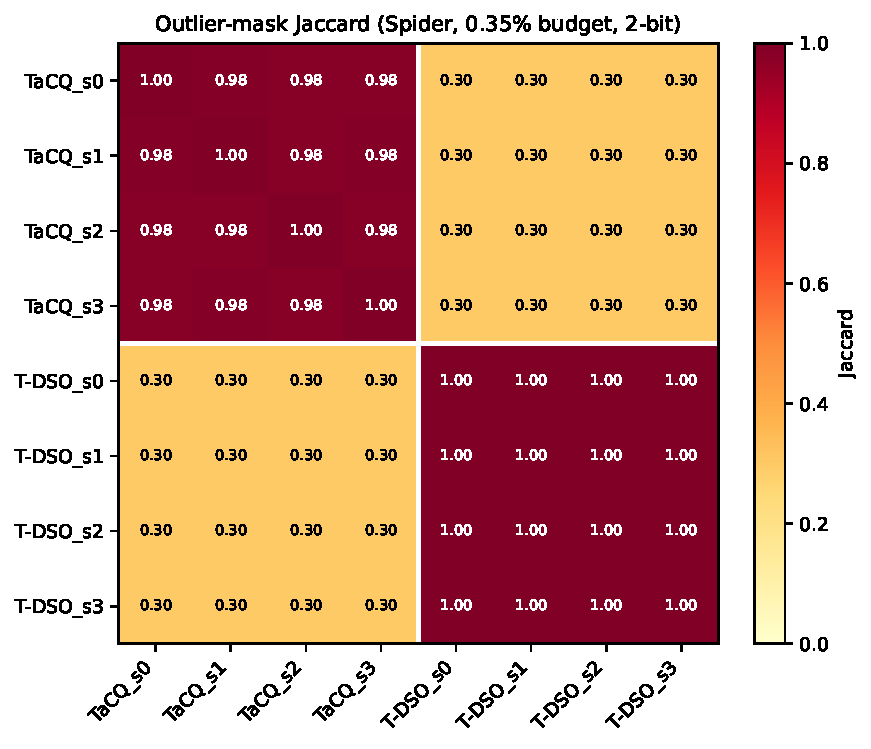
\includegraphics[width=0.7\linewidth]{figures/jaccard_matrix.pdf}
\caption{Cross-seed and cross-method Jaccard among 0.35\% outlier masks
(Spider, 2-bit). Diagonal blocks: within-method seeds ($J{>}0.98$);
off-diagonal: method gap ($J{\approx}0.30$).}
\label{fig:jaccard-matrix}
\end{figure}

\begin{figure}[t]
\centering
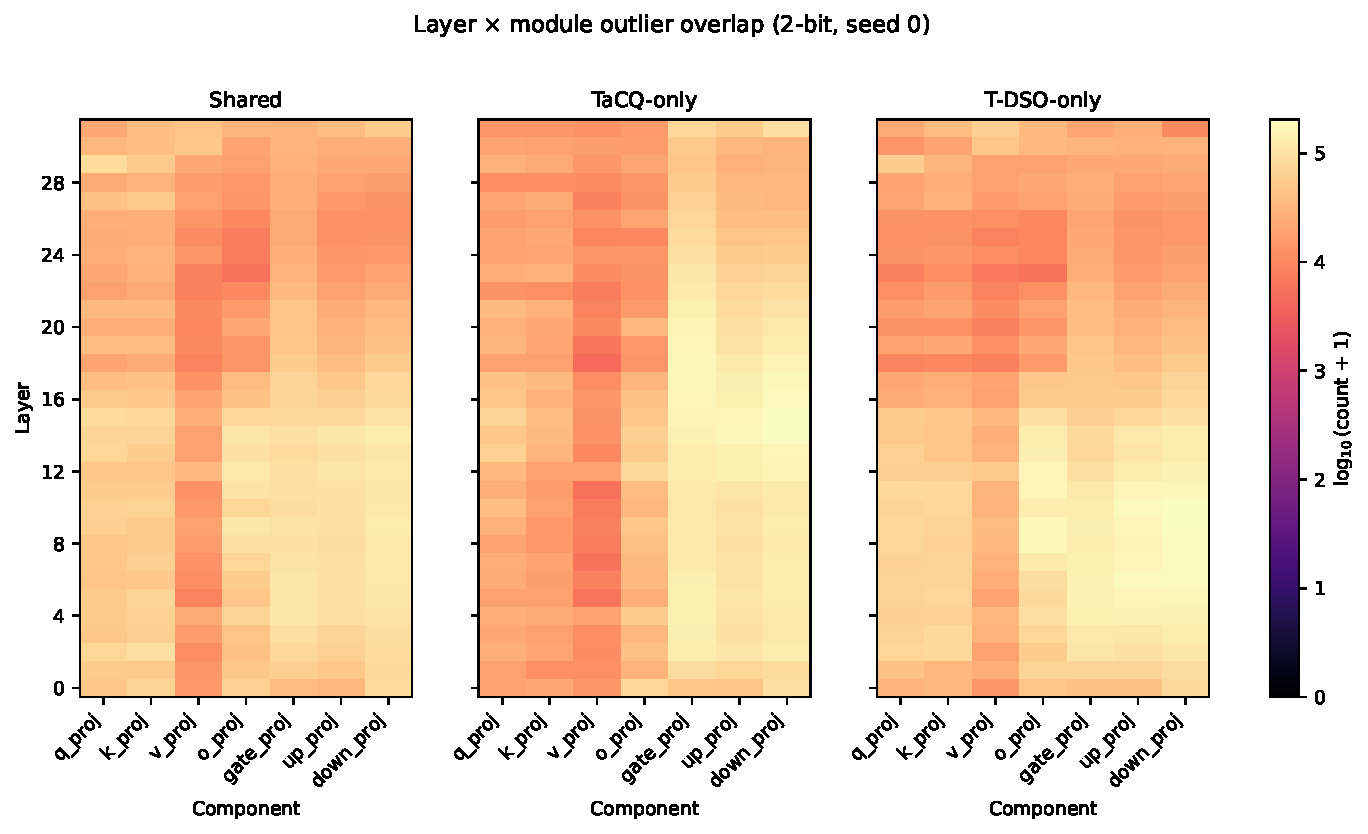
\includegraphics[width=0.9\linewidth]{figures/layer_module_heatmap.pdf}
\caption{Layer $\times$ module outlier decomposition (2-bit, seed 0): shared,
\baseline{}-only, and \method{}-only kept weights.}
\label{fig:layer-module}
\end{figure}

\subsection{Causal validation via targeted suppression}
\label{sec:analysis-knockout}

Scaling the 24.4M \method{}-masked weights by $\alpha{=}0.8$ on the FP16 model
(no quantization) drops Spider exec from 67.8\% to 38.9\% while short non-SQL
English probes remain fluent; the boost control ($\alpha{=}1.2$) also hurts
($-8.2$\,pt). The task-selective failure mode rules out the null that the mask
tags generic high-magnitude weights. A leak-free contrastive squeeze
($\alpha_{\text{task}}{=}1.05$, $\alpha_{\text{base}}{=}0.98$, selected on a
train holdout) yields $+1.0$\,pt dev exec over contemporaneous FP16.

\subsection{Why the native basis can beat the dictionary}
\label{sec:analysis-basis}

The MMLU-STEM reversal (mult$_{\text{free}}$ 44.2 vs.\ mult 38.9;
Table~\ref{tab:ablation}) suggests dictionary quality is task-dependent. Two
non-exclusive explanations: (i) \emph{coverage} --- CRV transcoders are trained
to reconstruct instruct-model MLP behavior on broad data; features that tile
mathematical CoT structure (GSM8K) may be better resolved than the
fine-grained factual retrieval MMLU stresses, so the transcoder's $\Delta a$
filter passes a noisier task set on MMLU; (ii) \emph{reconstruction error} ---
the alignment loss targets the transcoder's \emph{approximation} of the MLP
output; where reconstruction is weak, gradients partially chase approximation
artifacts. The native basis has zero reconstruction error by construction
(its decoder \emph{is} \texttt{down\_proj}), trading monosemanticity for
faithfulness. The conjunction with CE then filters its polysemantic noise.
This trade-off predicts the dictionary helps where its training distribution
matches the task and the native basis is safer elsewhere---a testable
criterion for future dictionary-aware PTQ.

\subsection{Efficiency and failure modes}
Saliency extraction matches \baseline{} asymptotics; the transcoder basis adds
per-layer encode/decode, the native basis adds only forward hooks. Union-style
combinations ($g_{\text{CE}}(1+\lambda g_{\text{align}})$) degenerate at 2-bit
(model rambles, no EOS), confirming that \emph{expanding} the CE mask with
circuit bonuses is worse than \emph{intersecting} the signals.

\section{Limitations}
\label{sec:limitations}

\begin{itemize}
  \item \textbf{Dictionary variant coverage.} Full per-layer CRV transcoders
        exist only for Llama-3.1-8B. The dictionary-free variant
        (\methodfree{}) removes this dependency for the method itself, but our
        cross-basis comparison (transcoder vs.\ native) is correspondingly
        limited to this model; replicating the basis--task interaction on a
        second model family is in progress.
  \item \textbf{Approximate MLP targets (transcoder basis).} TopK transcoders
        reconstruct MLP output imperfectly; where reconstruction is weak the
        alignment gradient partially chases approximation artifacts
        (\S\ref{sec:analysis-basis}). The native basis avoids this by
        construction.
  \item \textbf{Seed / calibration variance.} Both methods vary with
        calibration seed at 2-bit (Spider: \method{} spans 26.2--32.6\%, \baseline{}
        25.0--29.6\%). We report paired multi-seed means; single-seed entries
        are marked. Paired bootstrap confidence intervals are pending.
  \item \textbf{Task coverage.} Firm evidence on Spider, GSM8K, and three MMLU
        splits; HumanEval and broader reasoning suites are future work.
  \item \textbf{Scale.} Results are on an 8B model. The dictionary-free
        variant makes scale extension independent of dictionary releases;
        70B validation is queued.
\end{itemize}

\section{Systems Outlook: Dynamic Sparse Overlays}
\label{sec:systems-outlook}

Beyond static PTQ comparison, \method{} motivates a \textbf{Dynamic Sparse Overlay} execution model
not available to \baseline{}.
We do \emph{not} claim these systems results in v1; they define the research arc if v1 dissociation
holds empirically.

\paragraph{Agentic hot-swapping.}
\baseline{} produces one task-conditioned mask baked into the quantized checkpoint---configuration is
fixed for the inference job.
If sub-skills (schema linking, SQL generation, self-correction) prefer different outlier sets,
\baseline{} must compromise with a single global top-$k$.
\method{}'s feature-space objective naturally supports \emph{separate calibration streams} per
sub-skill and, with an orthogonality penalty on mask overlap, non-redundant overlays
$M_{\text{link}}$, $M_{\text{gen}}$, $M_{\text{fix}}$.
At runtime, only the FP16 outlier values differ; the 2-bit base $W_{\text{2bit}}$ stays resident while
overlay tables stream (e.g., via PCIe into on-chip SRAM).
\todo{Formalize QAL + orthogonality penalty; implement mask streaming benchmark.}

\paragraph{KV-cache inheritance.}
Multi-step text-to-SQL pipelines often chain agents as separate API calls.
Each call re-tokenizes history and recomputes attention from scratch---$O(N^2)$ per step.
With a shared frozen $W_{\text{2bit}}$ and hot-swapped overlays, a downstream sub-circuit inherits the
prior step's KV cache; only overlay weights and the active \method{} mask change.
Time-to-first-token for steps 2+ approaches cache-append cost rather than full prefill.
\todo{Microbenchmark TTFT: static TaCQ vs.\ overlay swap on two-step Spider prompt.}

\paragraph{Positioning for reviewers.}
Dimensions 2--3 are \emph{enabled by} feature dissociation plus mixed-precision structure; v1
validates Dimension 1 (Spider exec accuracy at matched budget).
Systems claims require separate engineering evidence and belong in an extended version or companion
systems section once built.

\section{Conclusion}
\label{sec:conclusion}

Low-bit PTQ forces a choice about which tiny fraction of weights must remain
in full precision. We started from an interpretability-guided answer---route
saliency through sparse transcoder features and intersect with the task loss
(\method{})---which beats \baseline{} at matched budget. Dissecting it with a
controlled ablation revealed the general principle underneath: protect a
weight only if it is salient to the task loss \emph{and} to the activation
circuit separating clean from corrupted task inputs, where the circuit can be
defined in the model's \emph{own} feature basis (\methodfree{}).

\paragraph{Three takeaways.}
\textbf{(1) The conjunction is the active ingredient.} In a controlled
saliency-source ablation with everything matched except the ranking signal,
the conjunction beats loss-only (CE/\baseline{}) and circuit-only selection on
both GSM8K and MMLU-STEM at 2-bit, and all circuit-informed arms dominate
magnitude/error/random controls by 10--26 points.
\textbf{(2) No dictionary required.} Computing the circuit term in the model's
own MLP-neuron basis (\methodfree{}) recovers most of the transcoder variant's
gain on GSM8K and surpasses it on MMLU-STEM---turning task-circuit PTQ from a
method gated on interpretability artifact releases into one that applies to
any transformer out-of-the-box.
\textbf{(3) Low-bit is where saliency matters.} At 3-bit all task-conditioned
methods converge to within seed noise; at 2-bit the saliency source separates
collapse from function. Mixed-precision PTQ research should therefore be
evaluated---and ablated---at the bit-widths where selection actually binds.

On Spider, intersecting CE with transcoder task-circuit attribution selects a
markedly different circuit ($J{=}0.30$ vs.\ \baseline{}) and improves 2-bit
execution accuracy by $+2.9$ points on average at matched budget, with causal
knockout supporting that the selected subnetwork implements task routing.

\paragraph{Future work.} Multi-task overlay masks
(\S\ref{sec:systems-outlook}), paired-bootstrap significance on all headline
gaps, second-model replication of the basis--task interaction, and
budget-fraction sweeps locating where the conjunction's advantage emerges.

\paragraph{Reproducibility.} Code, masks, contrastive calibration sets, and
replication logs: \todo{anonymous repo URL for submission}.


\bibliographystyle{plainnat}
\bibliography{references}

\appendix
\section{Hyperparameters}
\label{app:hyperparams}

\begin{table}[h]
\centering
\caption{Shared hyperparameters across \baseline{}, \method{}, and
\methodfree{}.}
\begin{tabular}{ll}
\toprule
Parameter & Value \\
\midrule
Outlier fraction & 0.35\% (global top-$k$) \\
Calibration pairs & 128 (Spider track: 1360) \\
Max sequence length & 2048 \\
Feature threshold quantile & 0.95 (per-example, positive $\Delta a$) \\
Transcoder TopK & 128 (\method{} only) \\
Native feature basis & MLP intermediate, $d_{\text{mlp}}{=}14{,}336$ (\methodfree{}) \\
GPTQ & true-sequential, 128 samples \\
$\Delta W$ reference & RTN $b$-bit (ablation) / GPTQ corrupt (Spider) \\
\bottomrule
\end{tabular}
\end{table}

\section{Contrastive corruption schema}
\label{app:corruptions}
Spider: schema swaps, wrong-SQL completions. GSM8K: corrupted chain-of-thought
with wrong intermediate steps and final answer. MMLU: wrong answer-choice
completions under the same 5-shot prompt.
\todo{full schema table from data\_prep\_contrastive.py}

\section{Saliency-source ablation: arm definitions}
\label{app:arms}
All arms share the mask format, 0.35\% global top-$k$ budget, GPTQ, and
evaluation. \textbf{random}: uniform random scores. \textbf{weight}: $|W|$.
\textbf{magnitude}: $|W|\cdot|\Delta W_{\text{RTN-}b\text{bit}}|$.
\textbf{ce}: $|W|\cdot|\Delta W|\cdot g_{\text{CE}}$. \textbf{align} /
\textbf{align$_{\text{free}}$}: $|W|\cdot|\Delta W|\cdot g_{\text{align}}$ in
the transcoder / native basis. \textbf{mult} / \textbf{mult$_{\text{free}}$}:
Eq.~\ref{eq:mult} in the transcoder / native basis.

\section{Transcoder-native feature audit}
\label{app:audit}
Per-layer task-feature density (\texttt{meta.layer\_feature\_density}) peaks in
mid layers 4--14, consistent with the layer-wise weight disagreement
(\S\ref{sec:analysis-overlap}). Top-K feature ranking by cumulative
clean$-$corrupt activation $\Delta a$ and manual labeling templates are
shipped with the code. \todo{populate manual labels}

\section{Additional results}
\label{app:additional}
\todo{Full Spider difficulty breakdown; complete dispute-sweep 2-bit row;
RTN vs.\ GPTQ $\Delta W$ ablation; cross-seed Jaccard tables.}

\section{Broader impact}
\label{app:impact}
Compression lowers the cost of deploying capable LLMs, which is dual-use in
the usual ways. Our interpretability-guided selection does not introduce new
capability risks beyond standard PTQ; it may improve auditability by making
the protected task circuit explicit.


\end{document}
